\documentclass[11pt]{article}
\usepackage[margin=1in]{geometry}
\usepackage{tikz}
\usetikzlibrary{arrows.meta,positioning,fit,backgrounds,calc,shapes.geometric}
\usepackage{amsmath,amssymb,booktabs,longtable,array,microtype,rotating}
\usepackage[hidelinks]{hyperref}
\usepackage{caption}
\captionsetup{font=small,labelfont=bf}
\newcommand{\nd}[1]{\ensuremath{#1}}
\newcommand{\obsmark}{\textsc{obs}}
\newcommand{\latmark}{\textsc{lat}}
\newcommand{\glbmark}{\textsc{glb}}
\title{A generative model of administrative process evidence}
\author{Regulatory complexity programme}
\date{}

\begin{document}
\maketitle

\section{What the model is for}

Given a statute and whatever the public can find about how some jurisdiction runs it, we want the
process: who does what, in what order, how long each step takes, what it costs, and which steps exist at
all. None of that is observed. What is observed is a pile of documents that disclose parts of it
selectively --- a programme page tells an applicant what to do and never mentions the back office; an
audit describes the back office and never mentions the fee; a forum post describes one person's wait.

The model below is the generative story for how that evidence comes to exist, so that inference can run
backwards from evidence to process. Two properties drive every design choice. First, \textbf{disclosure
is selective and the selection depends on the latent variable}: a step's visibility determines which
kinds of document mention it, so absence of evidence is informative and its strength depends on what
kind of document is silent. Second, \textbf{the observable is never the process}: it is a claim in a
document, or a duration someone reported, filtered through an extractor with its own error rate.

\begin{sidewaysfigure}[p]
  \centering
  \resizebox{\textheight}{!}{% Plate diagram: how an administrative process comes to be, and how evidence about it is generated.
% Hand-rolled node styles — no tikz-bayesnet dependency. Needs only:
%   \usetikzlibrary{arrows.meta,positioning,fit,backgrounds,calc,shapes.geometric}
% Use % Plate diagram: how an administrative process comes to be, and how evidence about it is generated.
% Hand-rolled node styles — no tikz-bayesnet dependency. Needs only:
%   \usetikzlibrary{arrows.meta,positioning,fit,backgrounds,calc,shapes.geometric}
% Use % Plate diagram: how an administrative process comes to be, and how evidence about it is generated.
% Hand-rolled node styles — no tikz-bayesnet dependency. Needs only:
%   \usetikzlibrary{arrows.meta,positioning,fit,backgrounds,calc,shapes.geometric}
% Use \input{plate_diagram.tex} inside a figure, or compile plate_diagram_standalone.tex.
%
% Layout notes: global parameters sit in the left and right margins, beside the plates they feed, so
% their edges stay short and horizontal instead of crossing the whole figure. Plate tags hang just
% below each plate rather than inside it, so they never collide with node captions.
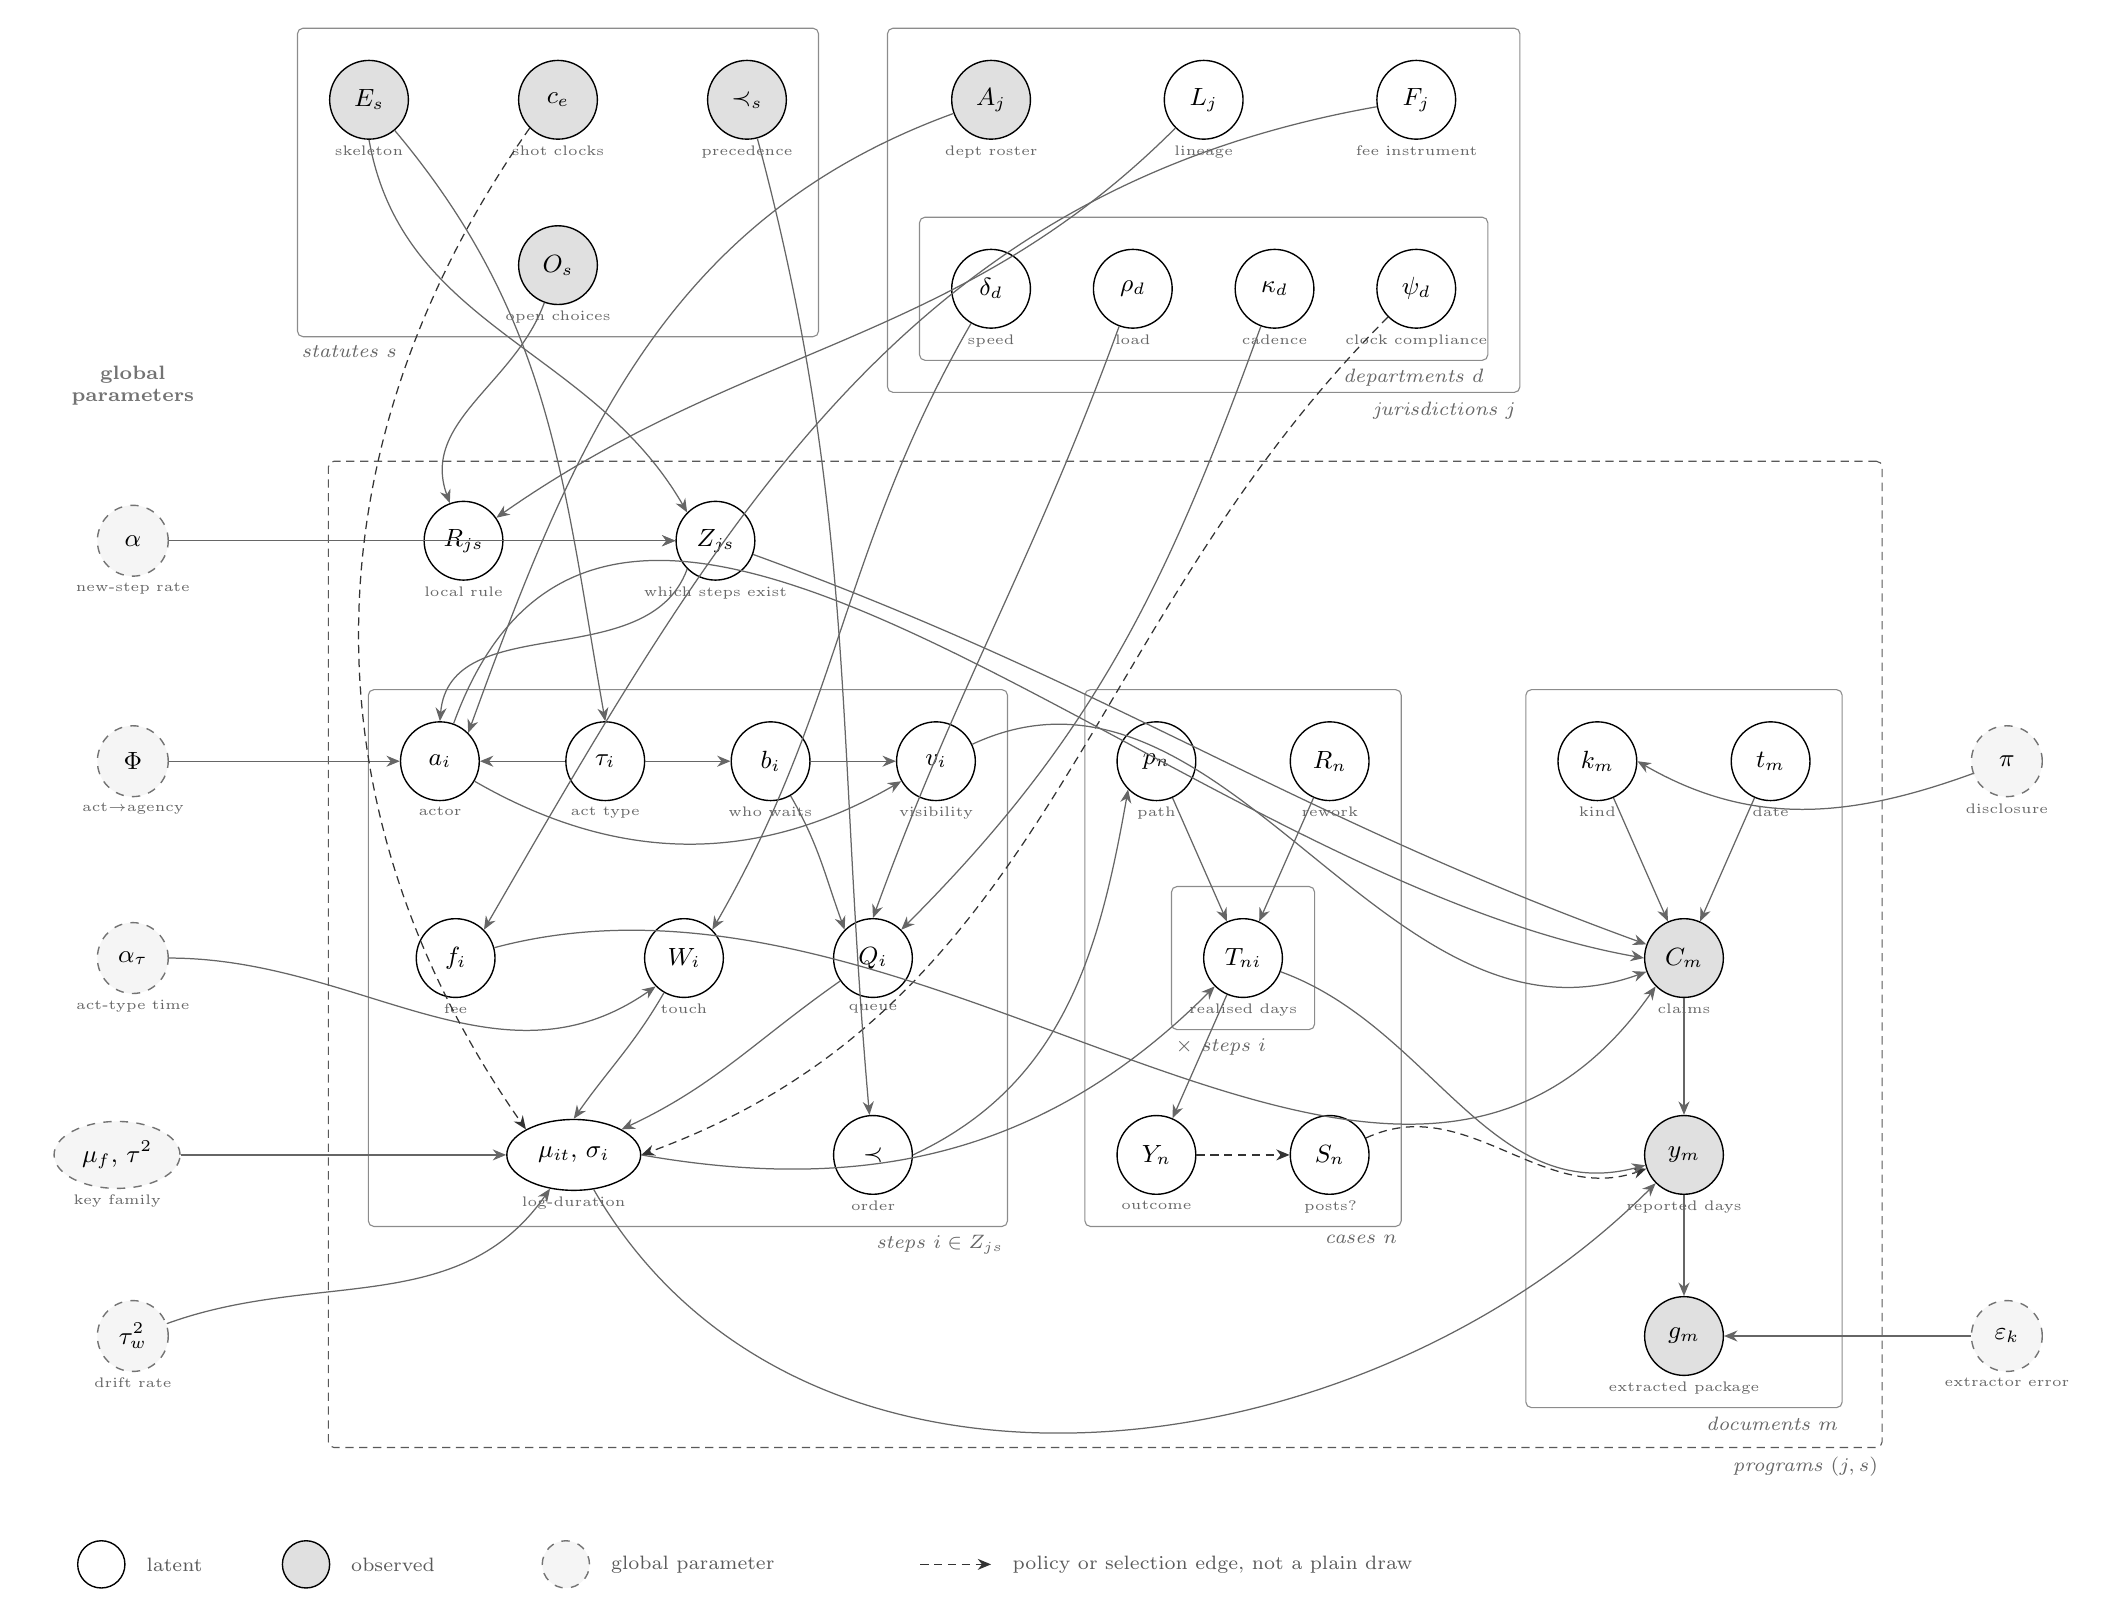
\begin{tikzpicture}[
  x=1cm, y=1cm,
  latent/.style = {circle, draw=black, line width=.5pt, fill=white,
                   minimum size=10mm, inner sep=.5pt, font=\small},
  obs/.style    = {latent, fill=black!12},
  hyper/.style  = {latent, fill=black!4, draw=black!55, dashed, minimum size=9mm},
  wide/.style   = {latent, ellipse, minimum width=17mm, minimum height=9mm},
  widehyp/.style= {hyper,  ellipse, minimum width=16mm, minimum height=8.5mm},
  lab/.style    = {font=\tiny, text=black!60, inner sep=1pt, text width=22mm, align=center},
  plate/.style  = {draw=black!45, rounded corners=2pt, inner sep=4mm, line width=.4pt},
  plate2/.style = {plate, densely dashed, draw=black!65, inner sep=5mm},
  ptag/.style   = {font=\scriptsize\itshape, text=black!60, inner sep=1.5pt},
  gtag/.style   = {font=\scriptsize\bfseries, text=black!55, align=center},
  ed/.style     = {-{Stealth[length=1.7mm,width=1.4mm]}, draw=black!60, line width=.45pt},
  sel/.style    = {ed, densely dashed, draw=black!80},
]

% ================= statute plate =================
\node[obs] (Es)   at ( 0.0, 0.0) {$E_s$};      \node[lab, below=1pt of Es]   {skeleton};
\node[obs] (ce)   at ( 2.4, 0.0) {$c_e$};      \node[lab, below=1pt of ce]   {shot clocks};
\node[obs] (prec) at ( 4.8, 0.0) {$\prec_s$};  \node[lab, below=1pt of prec] {precedence};
\node[obs] (Os)   at ( 2.4,-2.1) {$O_s$};      \node[lab, below=1pt of Os]   {open choices};

% ================= jurisdiction plate =================
\node[obs]    (Aj) at ( 7.9, 0.0) {$A_j$};  \node[lab, below=1pt of Aj] {dept roster};
\node[latent] (Lj) at (10.6, 0.0) {$L_j$};  \node[lab, below=1pt of Lj] {lineage};
\node[latent] (Fj) at (13.3, 0.0) {$F_j$};  \node[lab, below=1pt of Fj] {fee instrument};
\node[latent] (dd) at ( 7.9,-2.4) {$\delta_d$};  \node[lab, below=1pt of dd] {speed};
\node[latent] (rd) at ( 9.7,-2.4) {$\rho_d$};    \node[lab, below=1pt of rd] {load};
\node[latent] (kd) at (11.5,-2.4) {$\kappa_d$};  \node[lab, below=1pt of kd] {cadence};
\node[latent] (pd) at (13.3,-2.4) {$\psi_d$};    \node[lab, below=1pt of pd] {clock compliance};

% ================= program plate (j,s) =================
\node[latent] (Rjs) at ( 1.2,-5.6) {$R_{js}$};  \node[lab, below=1pt of Rjs] {local rule};
\node[latent] (Zjs) at ( 4.4,-5.6) {$Z_{js}$};  \node[lab, below=1pt of Zjs] {which steps exist};

% --- steps
\node[latent] (ai)  at ( 0.9,-8.4) {$a_i$};     \node[lab, below=1pt of ai]  {actor};
\node[latent] (ti)  at ( 3.0,-8.4) {$\tau_i$};  \node[lab, below=1pt of ti]  {act type};
\node[latent] (bi)  at ( 5.1,-8.4) {$b_i$};     \node[lab, below=1pt of bi]  {who waits};
\node[latent] (vi)  at ( 7.2,-8.4) {$v_i$};     \node[lab, below=1pt of vi]  {visibility};
\node[latent] (Qi)  at ( 6.4,-10.9) {$Q_i$};    \node[lab, below=1pt of Qi]  {queue};
\node[latent] (Wi)  at ( 4.0,-10.9) {$W_i$};    \node[lab, below=1pt of Wi]  {touch};
\node[latent] (fi)  at ( 1.1,-10.9) {$f_i$};    \node[lab, below=1pt of fi]  {fee};
\node[wide] (mui) at ( 2.6,-13.4) {$\mu_{it},\,\sigma_i$};
                                                 \node[lab, below=1pt of mui] {log-duration};
\node[latent] (ord) at ( 6.4,-13.4) {$\prec$};   \node[lab, below=1pt of ord] {order};

% --- cases
\node[latent] (pn)  at (10.0,-8.4)  {$p_n$};    \node[lab, below=1pt of pn] {path};
\node[latent] (Rn)  at (12.2,-8.4)  {$R_n$};    \node[lab, below=1pt of Rn] {rework};
\node[latent] (Tni) at (11.1,-10.9) {$T_{ni}$}; \node[lab, below=1pt of Tni] {realised days};
\node[latent] (Yn)  at (10.0,-13.4) {$Y_n$};    \node[lab, below=1pt of Yn] {outcome};
\node[latent] (Sn)  at (12.2,-13.4) {$S_n$};    \node[lab, below=1pt of Sn] {posts?};

% --- documents
\node[latent] (km) at (15.6,-8.4)  {$k_m$}; \node[lab, below=1pt of km] {kind};
\node[latent] (tm) at (17.8,-8.4)  {$t_m$}; \node[lab, below=1pt of tm] {date};
\node[obs]    (cm) at (16.7,-10.9) {$C_m$}; \node[lab, below=1pt of cm] {claims};
\node[obs]    (ym) at (16.7,-13.4) {$y_m$}; \node[lab, below=1pt of ym] {reported days};
\node[obs]    (gm) at (16.7,-15.7) {$g_m$}; \node[lab, below=1pt of gm] {extracted package};

% ================= plates =================
\begin{scope}[on background layer]
  \node[plate, fit=(Es)(ce)(prec)(Os)(Es.south)] (PS) {};
  \node[plate, fit=(dd)(rd)(kd)(pd)] (PD) {};
  \node[plate, fit=(Aj)(Lj)(Fj)(PD)] (PJ) {};
  \node[plate, fit=(Tni)] (PT) {};
  \node[plate, fit=(ai)(ti)(bi)(vi)(Qi)(Wi)(fi)(mui)(ord)] (PI) {};
  \node[plate, fit=(pn)(Rn)(PT)(Yn)(Sn)] (PN) {};
  \node[plate, fit=(km)(tm)(cm)(ym)(gm)] (PM) {};
  \node[plate2, fit=(Rjs)(Zjs)(PI)(PN)(PM)] (PP) {};
\end{scope}
% tags hang below their plate, never over a caption
\node[ptag, anchor=north west] at ($(PS.south west)+(0,-.5mm)$) {statutes $s$};
\node[ptag, anchor=north east] at ($(PD.south east)+(0,-.5mm)$) {departments $d$};
\node[ptag, anchor=north east] at ($(PJ.south east)+(0,-.5mm)$) {jurisdictions $j$};
\node[ptag, anchor=north west] at ($(PT.south west)+(0,-.5mm)$) {$\times$ steps $i$};
\node[ptag, anchor=north east] at ($(PI.south east)+(0,-.5mm)$) {steps $i\in Z_{js}$};
\node[ptag, anchor=north east] at ($(PN.south east)+(0,-.5mm)$) {cases $n$};
\node[ptag, anchor=north east] at ($(PM.south east)+(0,-.5mm)$) {documents $m$};
\node[ptag, anchor=north east] at ($(PP.south east)+(0,-.5mm)$)
     {programs $(j,s)$};

% ================= global parameters, in the margins beside what they feed =================
\node[gtag, anchor=south] at (-3.0,-4.0) {global\\parameters};
\node[hyper] (acrp) at (-3.0,-5.6)  {$\alpha$};        \node[lab, below=1pt of acrp] {new-step rate};
\node[hyper] (phi)  at (-3.0,-8.4)  {$\Phi$};          \node[lab, below=1pt of phi]  {act$\to$agency};
\node[hyper] (atau) at (-3.0,-10.9) {$\alpha_\tau$};   \node[lab, below=1pt of atau] {act-type time};
\node[widehyp] (mfam) at (-3.2,-13.4) {$\mu_f,\,\tau^2$}; \node[lab, below=1pt of mfam] {key family};
\node[hyper] (twk)  at (-3.0,-15.7) {$\tau^2_w$};      \node[lab, below=1pt of twk]  {drift rate};
\node[hyper] (pi)   at (20.8,-8.4)  {$\pi$};           \node[lab, below=1pt of pi]   {disclosure};
\node[hyper] (eps)  at (20.8,-15.7) {$\varepsilon_k$}; \node[lab, below=1pt of eps]  {extractor error};

% ================= edges =================
% statute / jurisdiction -> program
\draw[ed] (Os)  to[out=250,in=110] (Rjs);
\draw[ed] (Lj)  to[out=225,in=35]  (Rjs);
\draw[ed] (Es.south) to[out=280,in=120] (Zjs.north west);
\draw[ed] (Es)  to[out=310,in=100] (ti.north);          % the element fixes the kind of act
\draw[ed] (acrp) -- (Zjs.west);
\draw[ed] (Rjs) -- (Zjs);
\draw[ed] (Zjs.south west) to[out=250,in=85] (ai.north);

% actor
\draw[ed] (phi) -- (ai);
\draw[ed] (Aj)  to[out=200,in=70] (ai.north east);
\draw[ed] (ti)  -- (ai);
\draw[ed] (ti)  -- (bi);
\draw[ed] (ai)  to[out=330,in=210] (vi);
\draw[ed] (bi)  -- (vi);

% duration
\draw[ed] (atau) to[out=0,in=215] (Wi.south west);
\draw[ed] (dd)  to[out=240,in=60]  (Wi.north east);
\draw[ed] (rd)  to[out=250,in=70]  (Qi.north);
\draw[ed] (kd)  to[out=250,in=45]  (Qi.north east);
\draw[ed] (bi)  to[out=300,in=110] (Qi.north west);
\draw[ed] (Qi)  to[out=215,in=25]  (mui.north east);
\draw[ed] (Wi)  to[out=240,in=55]  (mui.north);
\draw[ed] (mfam) -- (mui);
\draw[ed] (twk) to[out=20,in=235]  (mui);
\draw[sel] (ce.south west) to[out=235,in=125] (mui.north west);
\draw[sel] (pd) to[out=225,in=20]  (mui.east);
\draw[ed] (Fj)  to[out=190,in=60]  (fi.north east);
\draw[ed] (prec) to[out=285,in=95] (ord);

% cases
\draw[ed] (ord.east) to[out=25,in=260] (pn.south west);
\draw[ed] (mui.east) to[out=350,in=225] (Tni.south west);
\draw[ed] (pn)  -- (Tni);
\draw[ed] (Rn)  -- (Tni);
\draw[ed] (Tni) -- (Yn);
\draw[sel] (Yn) -- (Sn);
\draw[sel] (Sn) to[out=25,in=200]  (ym);

% documents
\draw[ed] (vi)  to[out=25,in=200]  (cm);
\draw[ed] (fi)  to[out=15,in=235]  (cm.south west);   % a fee schedule states the fee
\draw[ed] (ai)  to[out=70,in=170]  (cm.west);          % and 36% of steps have their actor stated
\draw[ed] (Zjs) to[out=340,in=160] (cm);
\draw[ed] (pi)  to[out=200,in=330] (km.east);
\draw[ed] (km)  -- (cm);
\draw[ed] (tm)  -- (cm);
\draw[ed] (Tni) to[out=340,in=195] (ym);
\draw[ed] (cm)  -- (ym);
\draw[ed] (mui) to[out=300,in=225] (ym.south west);    % an official median describes mu, not a case
\draw[ed] (ym)  -- (gm);
\draw[ed] (eps) -- (gm);

% ================= legend =================
\begin{scope}[shift={(-3.4,-18.6)}]
  \node[latent, minimum size=6mm] (L1) at (0,0) {};
  \node[font=\scriptsize, text=black!65, anchor=west] at (0.45,0) {latent};
  \node[obs, minimum size=6mm] (L2) at (2.6,0) {};
  \node[font=\scriptsize, text=black!65, anchor=west] at (3.05,0) {observed};
  \node[hyper, minimum size=6mm] (L3) at (5.9,0) {};
  \node[font=\scriptsize, text=black!65, anchor=west] at (6.35,0) {global parameter};
  \draw[sel] (10.4,0) -- (11.3,0);
  \node[font=\scriptsize, text=black!65, anchor=west] at (11.45,0)
       {policy or selection edge, not a plain draw};
\end{scope}
\end{tikzpicture}
 inside a figure, or compile plate_diagram_standalone.tex.
%
% Layout notes: global parameters sit in the left and right margins, beside the plates they feed, so
% their edges stay short and horizontal instead of crossing the whole figure. Plate tags hang just
% below each plate rather than inside it, so they never collide with node captions.
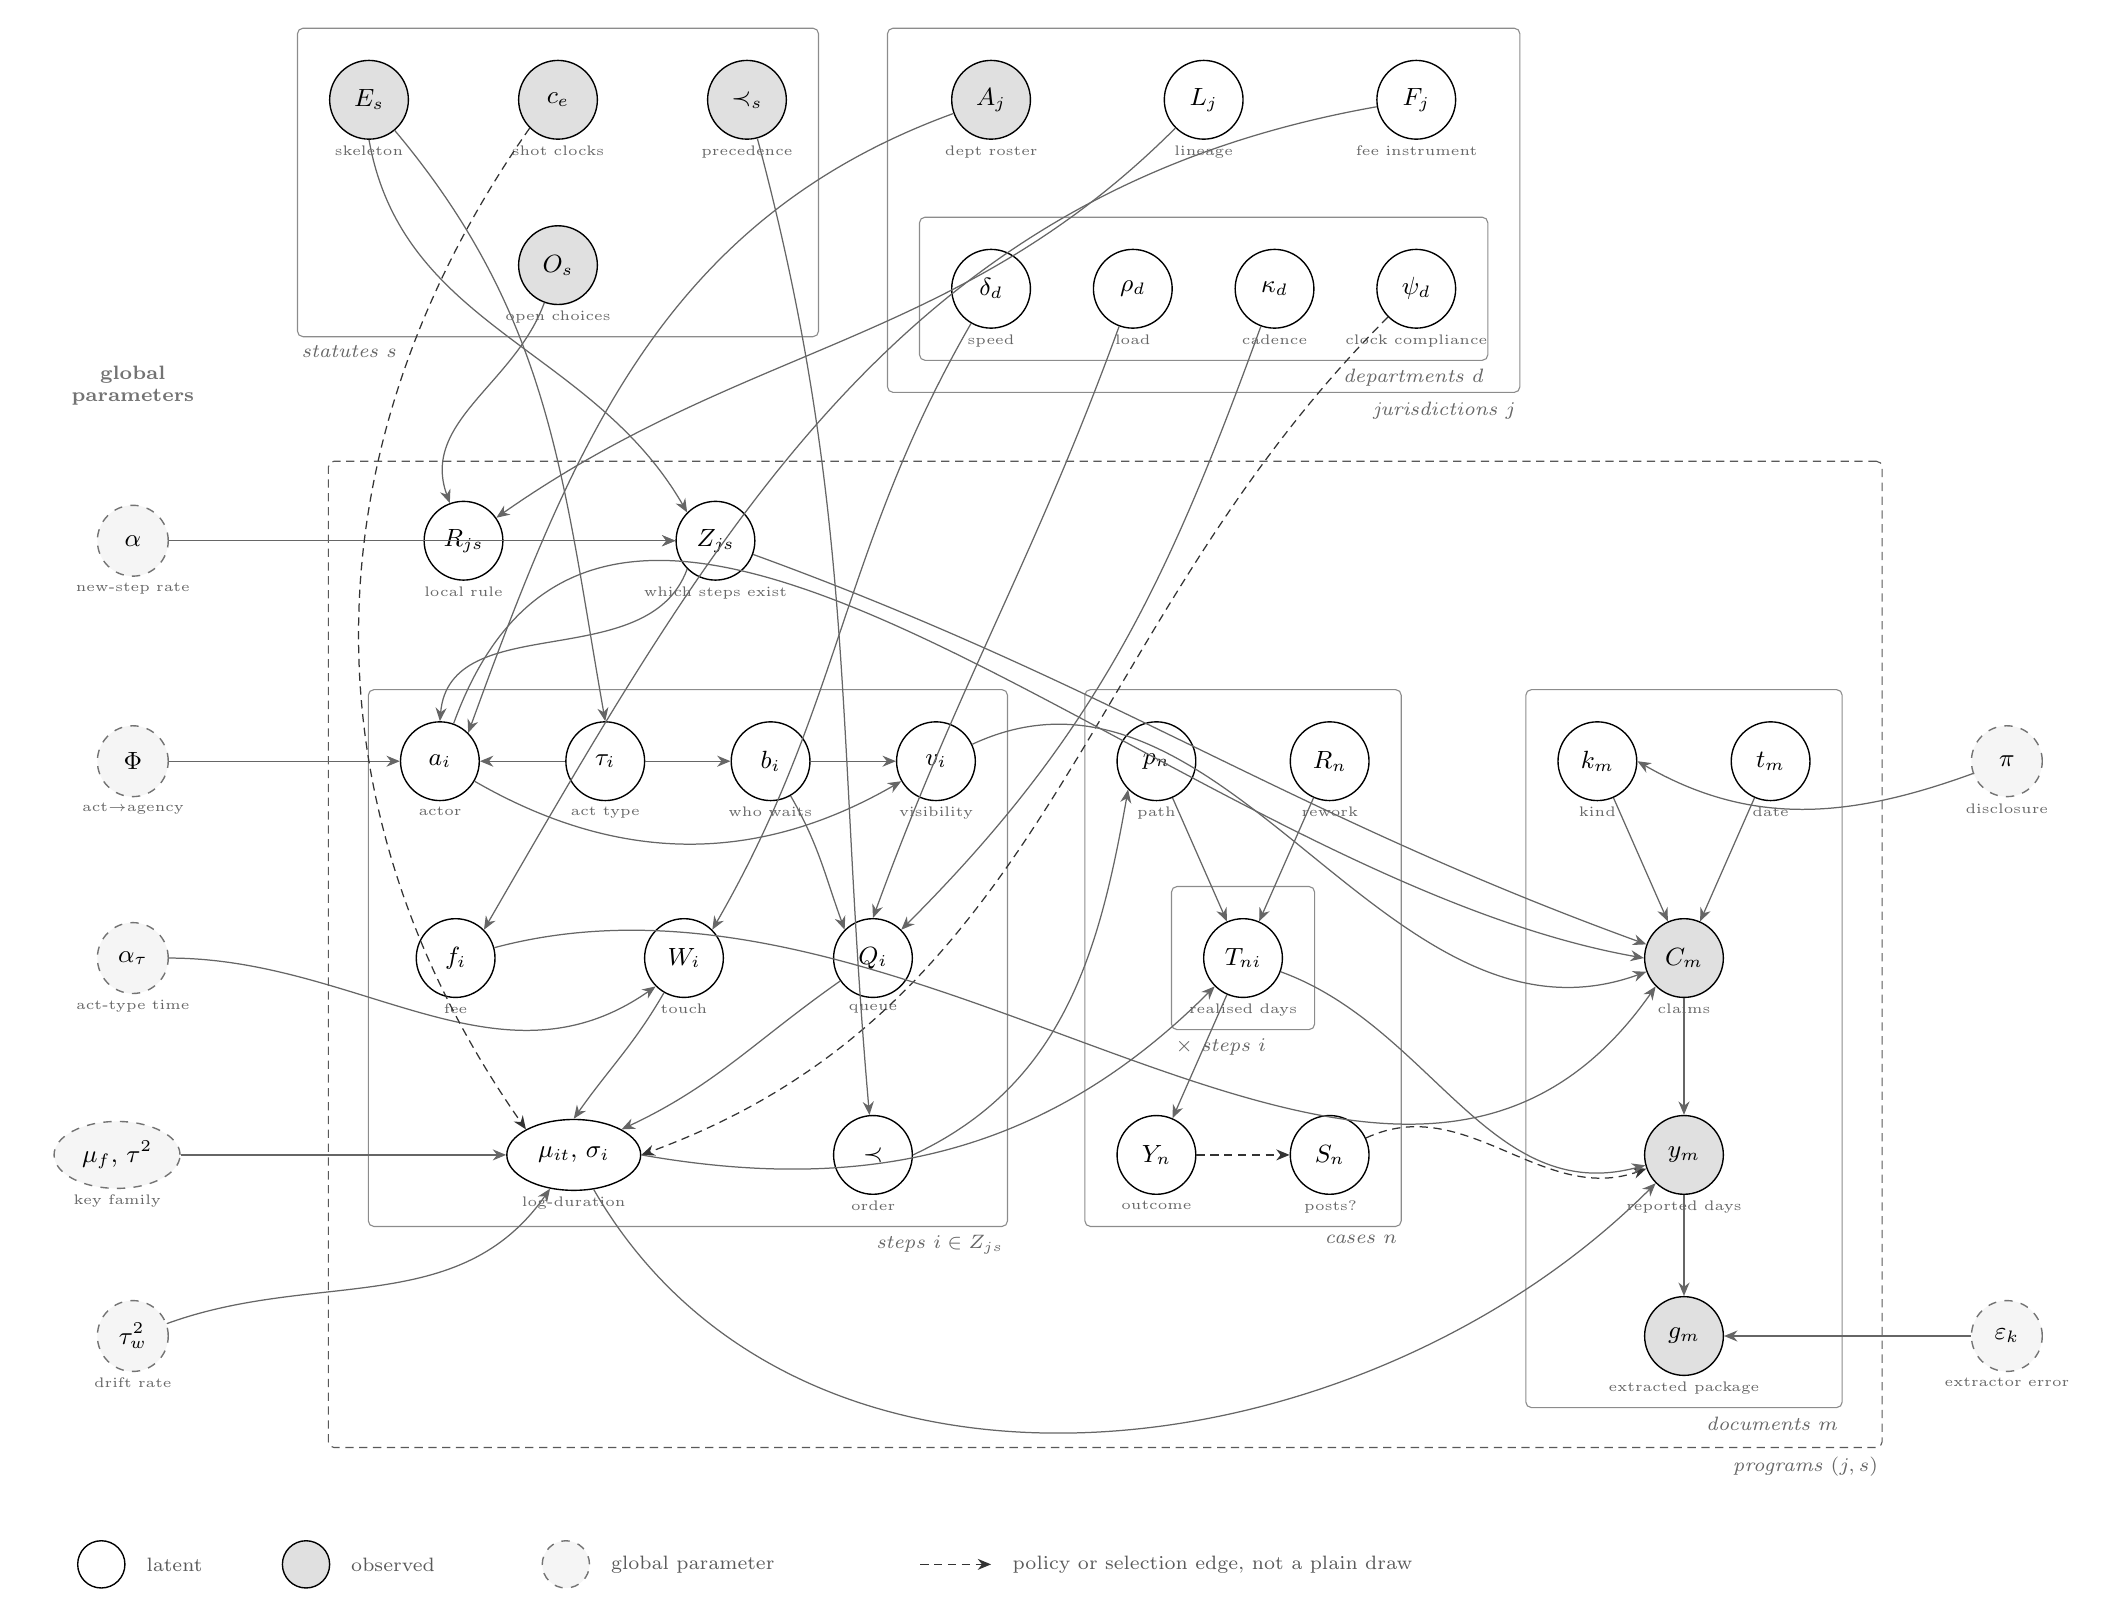
\begin{tikzpicture}[
  x=1cm, y=1cm,
  latent/.style = {circle, draw=black, line width=.5pt, fill=white,
                   minimum size=10mm, inner sep=.5pt, font=\small},
  obs/.style    = {latent, fill=black!12},
  hyper/.style  = {latent, fill=black!4, draw=black!55, dashed, minimum size=9mm},
  wide/.style   = {latent, ellipse, minimum width=17mm, minimum height=9mm},
  widehyp/.style= {hyper,  ellipse, minimum width=16mm, minimum height=8.5mm},
  lab/.style    = {font=\tiny, text=black!60, inner sep=1pt, text width=22mm, align=center},
  plate/.style  = {draw=black!45, rounded corners=2pt, inner sep=4mm, line width=.4pt},
  plate2/.style = {plate, densely dashed, draw=black!65, inner sep=5mm},
  ptag/.style   = {font=\scriptsize\itshape, text=black!60, inner sep=1.5pt},
  gtag/.style   = {font=\scriptsize\bfseries, text=black!55, align=center},
  ed/.style     = {-{Stealth[length=1.7mm,width=1.4mm]}, draw=black!60, line width=.45pt},
  sel/.style    = {ed, densely dashed, draw=black!80},
]

% ================= statute plate =================
\node[obs] (Es)   at ( 0.0, 0.0) {$E_s$};      \node[lab, below=1pt of Es]   {skeleton};
\node[obs] (ce)   at ( 2.4, 0.0) {$c_e$};      \node[lab, below=1pt of ce]   {shot clocks};
\node[obs] (prec) at ( 4.8, 0.0) {$\prec_s$};  \node[lab, below=1pt of prec] {precedence};
\node[obs] (Os)   at ( 2.4,-2.1) {$O_s$};      \node[lab, below=1pt of Os]   {open choices};

% ================= jurisdiction plate =================
\node[obs]    (Aj) at ( 7.9, 0.0) {$A_j$};  \node[lab, below=1pt of Aj] {dept roster};
\node[latent] (Lj) at (10.6, 0.0) {$L_j$};  \node[lab, below=1pt of Lj] {lineage};
\node[latent] (Fj) at (13.3, 0.0) {$F_j$};  \node[lab, below=1pt of Fj] {fee instrument};
\node[latent] (dd) at ( 7.9,-2.4) {$\delta_d$};  \node[lab, below=1pt of dd] {speed};
\node[latent] (rd) at ( 9.7,-2.4) {$\rho_d$};    \node[lab, below=1pt of rd] {load};
\node[latent] (kd) at (11.5,-2.4) {$\kappa_d$};  \node[lab, below=1pt of kd] {cadence};
\node[latent] (pd) at (13.3,-2.4) {$\psi_d$};    \node[lab, below=1pt of pd] {clock compliance};

% ================= program plate (j,s) =================
\node[latent] (Rjs) at ( 1.2,-5.6) {$R_{js}$};  \node[lab, below=1pt of Rjs] {local rule};
\node[latent] (Zjs) at ( 4.4,-5.6) {$Z_{js}$};  \node[lab, below=1pt of Zjs] {which steps exist};

% --- steps
\node[latent] (ai)  at ( 0.9,-8.4) {$a_i$};     \node[lab, below=1pt of ai]  {actor};
\node[latent] (ti)  at ( 3.0,-8.4) {$\tau_i$};  \node[lab, below=1pt of ti]  {act type};
\node[latent] (bi)  at ( 5.1,-8.4) {$b_i$};     \node[lab, below=1pt of bi]  {who waits};
\node[latent] (vi)  at ( 7.2,-8.4) {$v_i$};     \node[lab, below=1pt of vi]  {visibility};
\node[latent] (Qi)  at ( 6.4,-10.9) {$Q_i$};    \node[lab, below=1pt of Qi]  {queue};
\node[latent] (Wi)  at ( 4.0,-10.9) {$W_i$};    \node[lab, below=1pt of Wi]  {touch};
\node[latent] (fi)  at ( 1.1,-10.9) {$f_i$};    \node[lab, below=1pt of fi]  {fee};
\node[wide] (mui) at ( 2.6,-13.4) {$\mu_{it},\,\sigma_i$};
                                                 \node[lab, below=1pt of mui] {log-duration};
\node[latent] (ord) at ( 6.4,-13.4) {$\prec$};   \node[lab, below=1pt of ord] {order};

% --- cases
\node[latent] (pn)  at (10.0,-8.4)  {$p_n$};    \node[lab, below=1pt of pn] {path};
\node[latent] (Rn)  at (12.2,-8.4)  {$R_n$};    \node[lab, below=1pt of Rn] {rework};
\node[latent] (Tni) at (11.1,-10.9) {$T_{ni}$}; \node[lab, below=1pt of Tni] {realised days};
\node[latent] (Yn)  at (10.0,-13.4) {$Y_n$};    \node[lab, below=1pt of Yn] {outcome};
\node[latent] (Sn)  at (12.2,-13.4) {$S_n$};    \node[lab, below=1pt of Sn] {posts?};

% --- documents
\node[latent] (km) at (15.6,-8.4)  {$k_m$}; \node[lab, below=1pt of km] {kind};
\node[latent] (tm) at (17.8,-8.4)  {$t_m$}; \node[lab, below=1pt of tm] {date};
\node[obs]    (cm) at (16.7,-10.9) {$C_m$}; \node[lab, below=1pt of cm] {claims};
\node[obs]    (ym) at (16.7,-13.4) {$y_m$}; \node[lab, below=1pt of ym] {reported days};
\node[obs]    (gm) at (16.7,-15.7) {$g_m$}; \node[lab, below=1pt of gm] {extracted package};

% ================= plates =================
\begin{scope}[on background layer]
  \node[plate, fit=(Es)(ce)(prec)(Os)(Es.south)] (PS) {};
  \node[plate, fit=(dd)(rd)(kd)(pd)] (PD) {};
  \node[plate, fit=(Aj)(Lj)(Fj)(PD)] (PJ) {};
  \node[plate, fit=(Tni)] (PT) {};
  \node[plate, fit=(ai)(ti)(bi)(vi)(Qi)(Wi)(fi)(mui)(ord)] (PI) {};
  \node[plate, fit=(pn)(Rn)(PT)(Yn)(Sn)] (PN) {};
  \node[plate, fit=(km)(tm)(cm)(ym)(gm)] (PM) {};
  \node[plate2, fit=(Rjs)(Zjs)(PI)(PN)(PM)] (PP) {};
\end{scope}
% tags hang below their plate, never over a caption
\node[ptag, anchor=north west] at ($(PS.south west)+(0,-.5mm)$) {statutes $s$};
\node[ptag, anchor=north east] at ($(PD.south east)+(0,-.5mm)$) {departments $d$};
\node[ptag, anchor=north east] at ($(PJ.south east)+(0,-.5mm)$) {jurisdictions $j$};
\node[ptag, anchor=north west] at ($(PT.south west)+(0,-.5mm)$) {$\times$ steps $i$};
\node[ptag, anchor=north east] at ($(PI.south east)+(0,-.5mm)$) {steps $i\in Z_{js}$};
\node[ptag, anchor=north east] at ($(PN.south east)+(0,-.5mm)$) {cases $n$};
\node[ptag, anchor=north east] at ($(PM.south east)+(0,-.5mm)$) {documents $m$};
\node[ptag, anchor=north east] at ($(PP.south east)+(0,-.5mm)$)
     {programs $(j,s)$};

% ================= global parameters, in the margins beside what they feed =================
\node[gtag, anchor=south] at (-3.0,-4.0) {global\\parameters};
\node[hyper] (acrp) at (-3.0,-5.6)  {$\alpha$};        \node[lab, below=1pt of acrp] {new-step rate};
\node[hyper] (phi)  at (-3.0,-8.4)  {$\Phi$};          \node[lab, below=1pt of phi]  {act$\to$agency};
\node[hyper] (atau) at (-3.0,-10.9) {$\alpha_\tau$};   \node[lab, below=1pt of atau] {act-type time};
\node[widehyp] (mfam) at (-3.2,-13.4) {$\mu_f,\,\tau^2$}; \node[lab, below=1pt of mfam] {key family};
\node[hyper] (twk)  at (-3.0,-15.7) {$\tau^2_w$};      \node[lab, below=1pt of twk]  {drift rate};
\node[hyper] (pi)   at (20.8,-8.4)  {$\pi$};           \node[lab, below=1pt of pi]   {disclosure};
\node[hyper] (eps)  at (20.8,-15.7) {$\varepsilon_k$}; \node[lab, below=1pt of eps]  {extractor error};

% ================= edges =================
% statute / jurisdiction -> program
\draw[ed] (Os)  to[out=250,in=110] (Rjs);
\draw[ed] (Lj)  to[out=225,in=35]  (Rjs);
\draw[ed] (Es.south) to[out=280,in=120] (Zjs.north west);
\draw[ed] (Es)  to[out=310,in=100] (ti.north);          % the element fixes the kind of act
\draw[ed] (acrp) -- (Zjs.west);
\draw[ed] (Rjs) -- (Zjs);
\draw[ed] (Zjs.south west) to[out=250,in=85] (ai.north);

% actor
\draw[ed] (phi) -- (ai);
\draw[ed] (Aj)  to[out=200,in=70] (ai.north east);
\draw[ed] (ti)  -- (ai);
\draw[ed] (ti)  -- (bi);
\draw[ed] (ai)  to[out=330,in=210] (vi);
\draw[ed] (bi)  -- (vi);

% duration
\draw[ed] (atau) to[out=0,in=215] (Wi.south west);
\draw[ed] (dd)  to[out=240,in=60]  (Wi.north east);
\draw[ed] (rd)  to[out=250,in=70]  (Qi.north);
\draw[ed] (kd)  to[out=250,in=45]  (Qi.north east);
\draw[ed] (bi)  to[out=300,in=110] (Qi.north west);
\draw[ed] (Qi)  to[out=215,in=25]  (mui.north east);
\draw[ed] (Wi)  to[out=240,in=55]  (mui.north);
\draw[ed] (mfam) -- (mui);
\draw[ed] (twk) to[out=20,in=235]  (mui);
\draw[sel] (ce.south west) to[out=235,in=125] (mui.north west);
\draw[sel] (pd) to[out=225,in=20]  (mui.east);
\draw[ed] (Fj)  to[out=190,in=60]  (fi.north east);
\draw[ed] (prec) to[out=285,in=95] (ord);

% cases
\draw[ed] (ord.east) to[out=25,in=260] (pn.south west);
\draw[ed] (mui.east) to[out=350,in=225] (Tni.south west);
\draw[ed] (pn)  -- (Tni);
\draw[ed] (Rn)  -- (Tni);
\draw[ed] (Tni) -- (Yn);
\draw[sel] (Yn) -- (Sn);
\draw[sel] (Sn) to[out=25,in=200]  (ym);

% documents
\draw[ed] (vi)  to[out=25,in=200]  (cm);
\draw[ed] (fi)  to[out=15,in=235]  (cm.south west);   % a fee schedule states the fee
\draw[ed] (ai)  to[out=70,in=170]  (cm.west);          % and 36% of steps have their actor stated
\draw[ed] (Zjs) to[out=340,in=160] (cm);
\draw[ed] (pi)  to[out=200,in=330] (km.east);
\draw[ed] (km)  -- (cm);
\draw[ed] (tm)  -- (cm);
\draw[ed] (Tni) to[out=340,in=195] (ym);
\draw[ed] (cm)  -- (ym);
\draw[ed] (mui) to[out=300,in=225] (ym.south west);    % an official median describes mu, not a case
\draw[ed] (ym)  -- (gm);
\draw[ed] (eps) -- (gm);

% ================= legend =================
\begin{scope}[shift={(-3.4,-18.6)}]
  \node[latent, minimum size=6mm] (L1) at (0,0) {};
  \node[font=\scriptsize, text=black!65, anchor=west] at (0.45,0) {latent};
  \node[obs, minimum size=6mm] (L2) at (2.6,0) {};
  \node[font=\scriptsize, text=black!65, anchor=west] at (3.05,0) {observed};
  \node[hyper, minimum size=6mm] (L3) at (5.9,0) {};
  \node[font=\scriptsize, text=black!65, anchor=west] at (6.35,0) {global parameter};
  \draw[sel] (10.4,0) -- (11.3,0);
  \node[font=\scriptsize, text=black!65, anchor=west] at (11.45,0)
       {policy or selection edge, not a plain draw};
\end{scope}
\end{tikzpicture}
 inside a figure, or compile plate_diagram_standalone.tex.
%
% Layout notes: global parameters sit in the left and right margins, beside the plates they feed, so
% their edges stay short and horizontal instead of crossing the whole figure. Plate tags hang just
% below each plate rather than inside it, so they never collide with node captions.
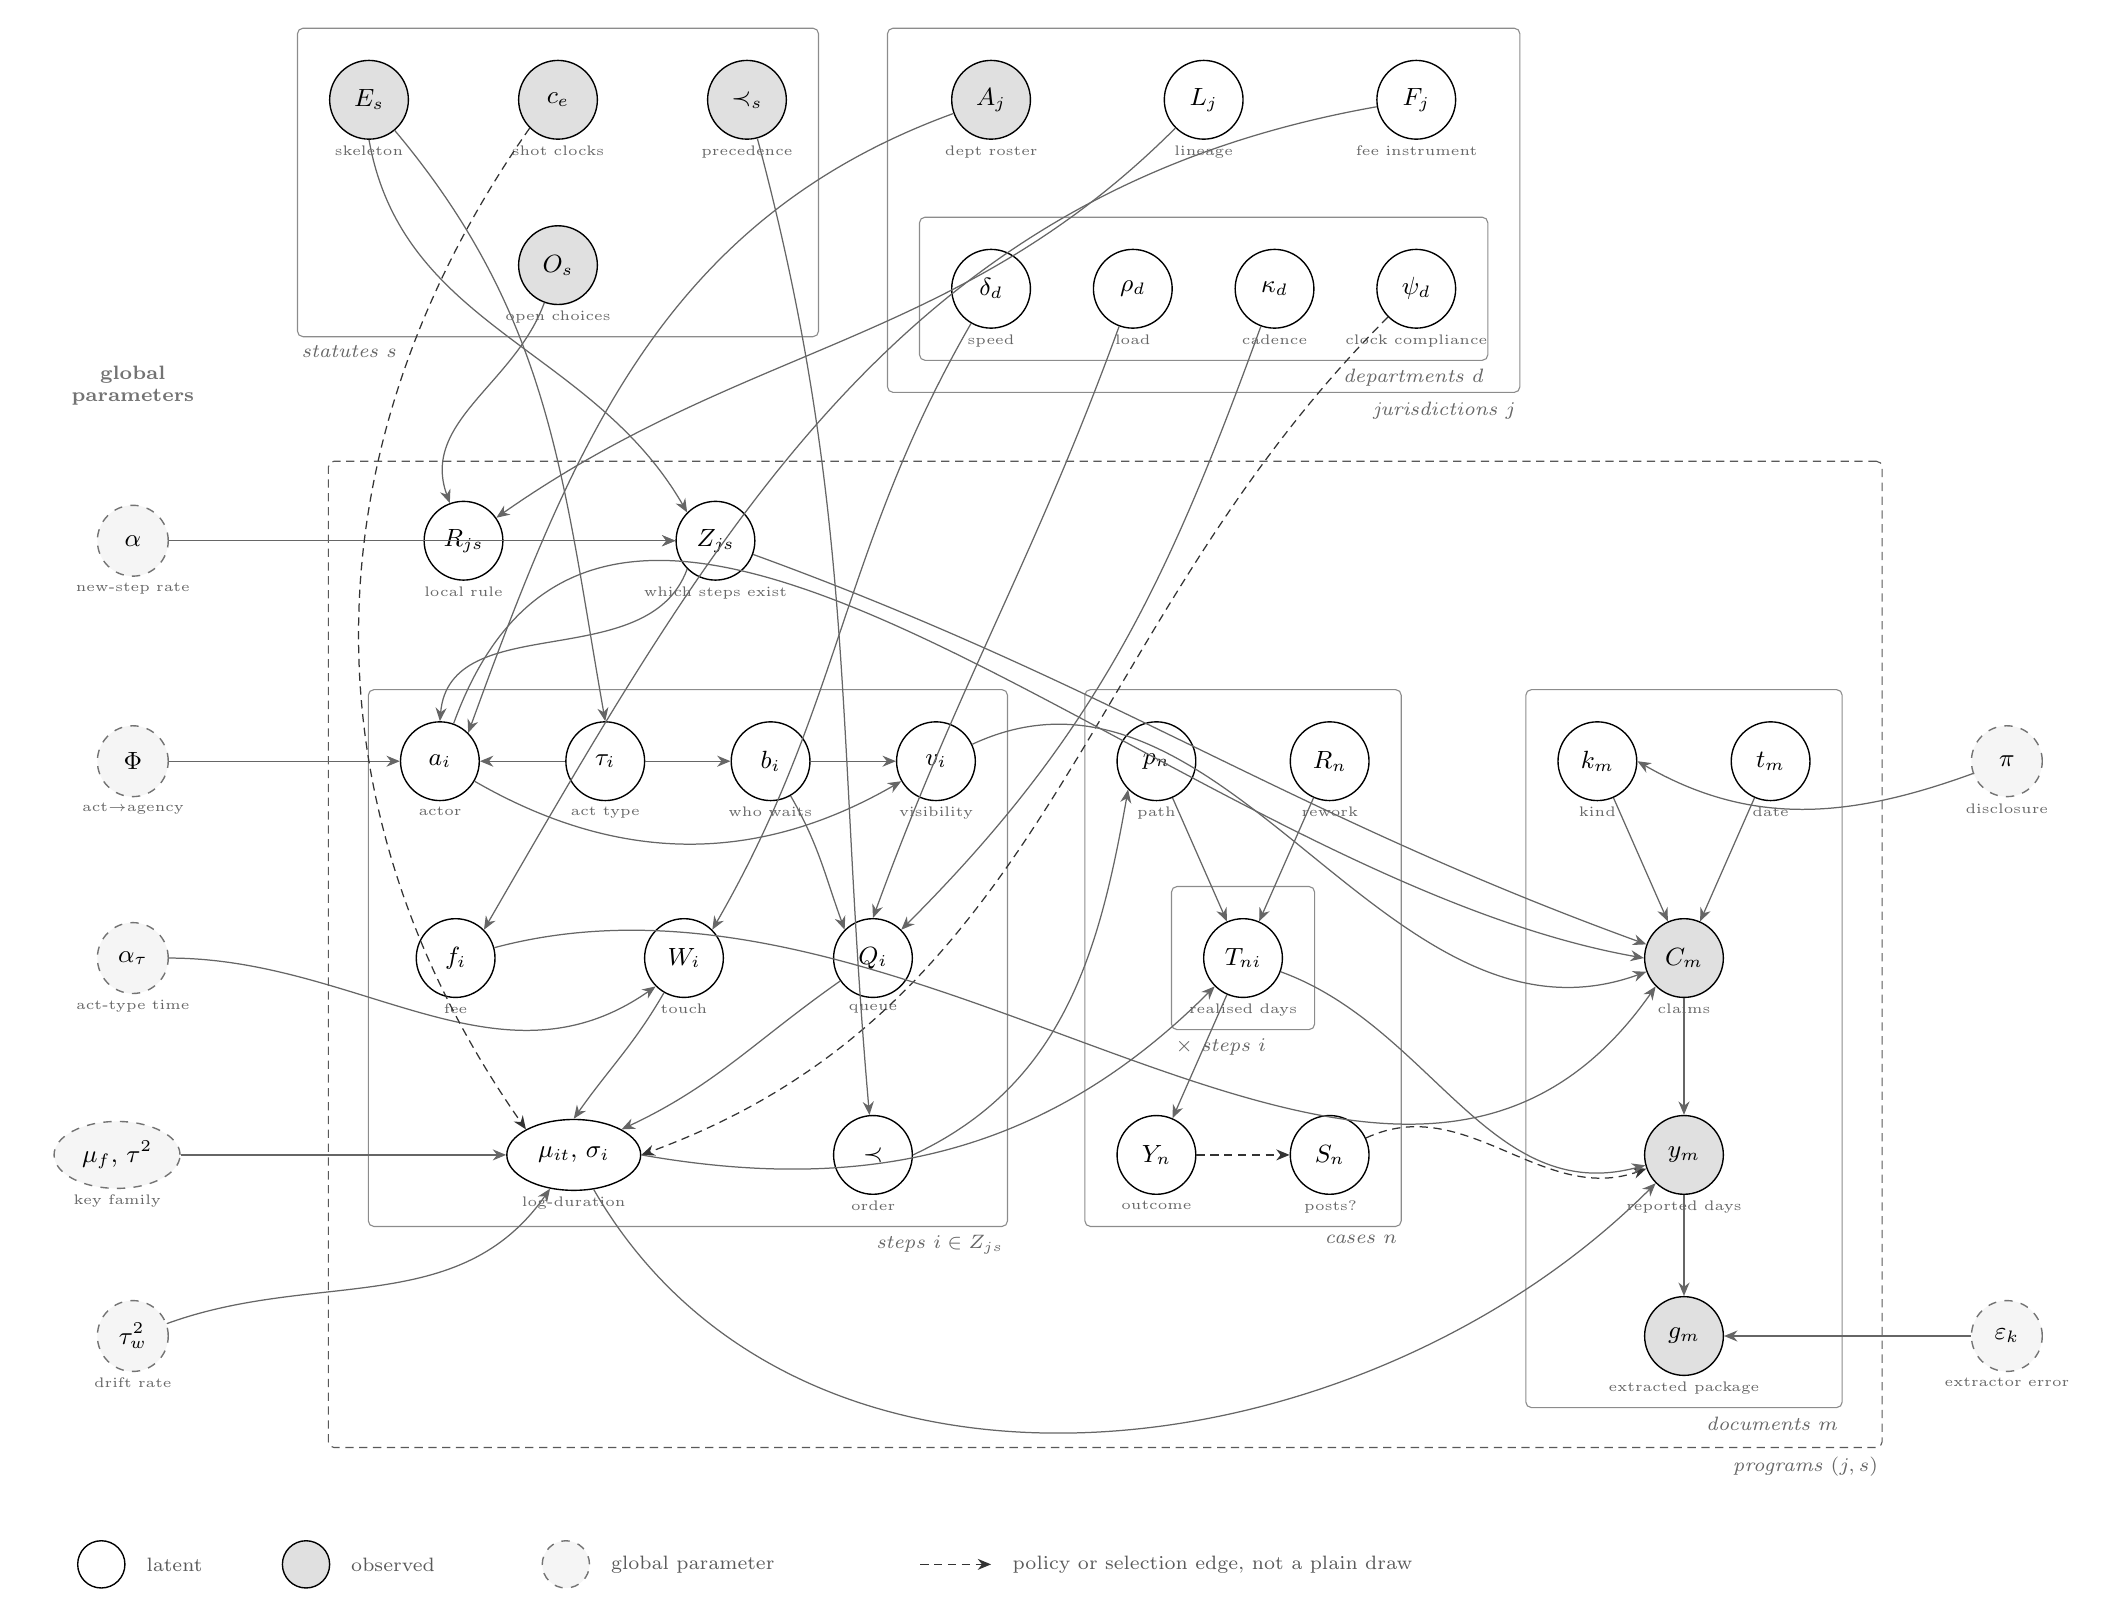
\begin{tikzpicture}[
  x=1cm, y=1cm,
  latent/.style = {circle, draw=black, line width=.5pt, fill=white,
                   minimum size=10mm, inner sep=.5pt, font=\small},
  obs/.style    = {latent, fill=black!12},
  hyper/.style  = {latent, fill=black!4, draw=black!55, dashed, minimum size=9mm},
  wide/.style   = {latent, ellipse, minimum width=17mm, minimum height=9mm},
  widehyp/.style= {hyper,  ellipse, minimum width=16mm, minimum height=8.5mm},
  lab/.style    = {font=\tiny, text=black!60, inner sep=1pt, text width=22mm, align=center},
  plate/.style  = {draw=black!45, rounded corners=2pt, inner sep=4mm, line width=.4pt},
  plate2/.style = {plate, densely dashed, draw=black!65, inner sep=5mm},
  ptag/.style   = {font=\scriptsize\itshape, text=black!60, inner sep=1.5pt},
  gtag/.style   = {font=\scriptsize\bfseries, text=black!55, align=center},
  ed/.style     = {-{Stealth[length=1.7mm,width=1.4mm]}, draw=black!60, line width=.45pt},
  sel/.style    = {ed, densely dashed, draw=black!80},
]

% ================= statute plate =================
\node[obs] (Es)   at ( 0.0, 0.0) {$E_s$};      \node[lab, below=1pt of Es]   {skeleton};
\node[obs] (ce)   at ( 2.4, 0.0) {$c_e$};      \node[lab, below=1pt of ce]   {shot clocks};
\node[obs] (prec) at ( 4.8, 0.0) {$\prec_s$};  \node[lab, below=1pt of prec] {precedence};
\node[obs] (Os)   at ( 2.4,-2.1) {$O_s$};      \node[lab, below=1pt of Os]   {open choices};

% ================= jurisdiction plate =================
\node[obs]    (Aj) at ( 7.9, 0.0) {$A_j$};  \node[lab, below=1pt of Aj] {dept roster};
\node[latent] (Lj) at (10.6, 0.0) {$L_j$};  \node[lab, below=1pt of Lj] {lineage};
\node[latent] (Fj) at (13.3, 0.0) {$F_j$};  \node[lab, below=1pt of Fj] {fee instrument};
\node[latent] (dd) at ( 7.9,-2.4) {$\delta_d$};  \node[lab, below=1pt of dd] {speed};
\node[latent] (rd) at ( 9.7,-2.4) {$\rho_d$};    \node[lab, below=1pt of rd] {load};
\node[latent] (kd) at (11.5,-2.4) {$\kappa_d$};  \node[lab, below=1pt of kd] {cadence};
\node[latent] (pd) at (13.3,-2.4) {$\psi_d$};    \node[lab, below=1pt of pd] {clock compliance};

% ================= program plate (j,s) =================
\node[latent] (Rjs) at ( 1.2,-5.6) {$R_{js}$};  \node[lab, below=1pt of Rjs] {local rule};
\node[latent] (Zjs) at ( 4.4,-5.6) {$Z_{js}$};  \node[lab, below=1pt of Zjs] {which steps exist};

% --- steps
\node[latent] (ai)  at ( 0.9,-8.4) {$a_i$};     \node[lab, below=1pt of ai]  {actor};
\node[latent] (ti)  at ( 3.0,-8.4) {$\tau_i$};  \node[lab, below=1pt of ti]  {act type};
\node[latent] (bi)  at ( 5.1,-8.4) {$b_i$};     \node[lab, below=1pt of bi]  {who waits};
\node[latent] (vi)  at ( 7.2,-8.4) {$v_i$};     \node[lab, below=1pt of vi]  {visibility};
\node[latent] (Qi)  at ( 6.4,-10.9) {$Q_i$};    \node[lab, below=1pt of Qi]  {queue};
\node[latent] (Wi)  at ( 4.0,-10.9) {$W_i$};    \node[lab, below=1pt of Wi]  {touch};
\node[latent] (fi)  at ( 1.1,-10.9) {$f_i$};    \node[lab, below=1pt of fi]  {fee};
\node[wide] (mui) at ( 2.6,-13.4) {$\mu_{it},\,\sigma_i$};
                                                 \node[lab, below=1pt of mui] {log-duration};
\node[latent] (ord) at ( 6.4,-13.4) {$\prec$};   \node[lab, below=1pt of ord] {order};

% --- cases
\node[latent] (pn)  at (10.0,-8.4)  {$p_n$};    \node[lab, below=1pt of pn] {path};
\node[latent] (Rn)  at (12.2,-8.4)  {$R_n$};    \node[lab, below=1pt of Rn] {rework};
\node[latent] (Tni) at (11.1,-10.9) {$T_{ni}$}; \node[lab, below=1pt of Tni] {realised days};
\node[latent] (Yn)  at (10.0,-13.4) {$Y_n$};    \node[lab, below=1pt of Yn] {outcome};
\node[latent] (Sn)  at (12.2,-13.4) {$S_n$};    \node[lab, below=1pt of Sn] {posts?};

% --- documents
\node[latent] (km) at (15.6,-8.4)  {$k_m$}; \node[lab, below=1pt of km] {kind};
\node[latent] (tm) at (17.8,-8.4)  {$t_m$}; \node[lab, below=1pt of tm] {date};
\node[obs]    (cm) at (16.7,-10.9) {$C_m$}; \node[lab, below=1pt of cm] {claims};
\node[obs]    (ym) at (16.7,-13.4) {$y_m$}; \node[lab, below=1pt of ym] {reported days};
\node[obs]    (gm) at (16.7,-15.7) {$g_m$}; \node[lab, below=1pt of gm] {extracted package};

% ================= plates =================
\begin{scope}[on background layer]
  \node[plate, fit=(Es)(ce)(prec)(Os)(Es.south)] (PS) {};
  \node[plate, fit=(dd)(rd)(kd)(pd)] (PD) {};
  \node[plate, fit=(Aj)(Lj)(Fj)(PD)] (PJ) {};
  \node[plate, fit=(Tni)] (PT) {};
  \node[plate, fit=(ai)(ti)(bi)(vi)(Qi)(Wi)(fi)(mui)(ord)] (PI) {};
  \node[plate, fit=(pn)(Rn)(PT)(Yn)(Sn)] (PN) {};
  \node[plate, fit=(km)(tm)(cm)(ym)(gm)] (PM) {};
  \node[plate2, fit=(Rjs)(Zjs)(PI)(PN)(PM)] (PP) {};
\end{scope}
% tags hang below their plate, never over a caption
\node[ptag, anchor=north west] at ($(PS.south west)+(0,-.5mm)$) {statutes $s$};
\node[ptag, anchor=north east] at ($(PD.south east)+(0,-.5mm)$) {departments $d$};
\node[ptag, anchor=north east] at ($(PJ.south east)+(0,-.5mm)$) {jurisdictions $j$};
\node[ptag, anchor=north west] at ($(PT.south west)+(0,-.5mm)$) {$\times$ steps $i$};
\node[ptag, anchor=north east] at ($(PI.south east)+(0,-.5mm)$) {steps $i\in Z_{js}$};
\node[ptag, anchor=north east] at ($(PN.south east)+(0,-.5mm)$) {cases $n$};
\node[ptag, anchor=north east] at ($(PM.south east)+(0,-.5mm)$) {documents $m$};
\node[ptag, anchor=north east] at ($(PP.south east)+(0,-.5mm)$)
     {programs $(j,s)$};

% ================= global parameters, in the margins beside what they feed =================
\node[gtag, anchor=south] at (-3.0,-4.0) {global\\parameters};
\node[hyper] (acrp) at (-3.0,-5.6)  {$\alpha$};        \node[lab, below=1pt of acrp] {new-step rate};
\node[hyper] (phi)  at (-3.0,-8.4)  {$\Phi$};          \node[lab, below=1pt of phi]  {act$\to$agency};
\node[hyper] (atau) at (-3.0,-10.9) {$\alpha_\tau$};   \node[lab, below=1pt of atau] {act-type time};
\node[widehyp] (mfam) at (-3.2,-13.4) {$\mu_f,\,\tau^2$}; \node[lab, below=1pt of mfam] {key family};
\node[hyper] (twk)  at (-3.0,-15.7) {$\tau^2_w$};      \node[lab, below=1pt of twk]  {drift rate};
\node[hyper] (pi)   at (20.8,-8.4)  {$\pi$};           \node[lab, below=1pt of pi]   {disclosure};
\node[hyper] (eps)  at (20.8,-15.7) {$\varepsilon_k$}; \node[lab, below=1pt of eps]  {extractor error};

% ================= edges =================
% statute / jurisdiction -> program
\draw[ed] (Os)  to[out=250,in=110] (Rjs);
\draw[ed] (Lj)  to[out=225,in=35]  (Rjs);
\draw[ed] (Es.south) to[out=280,in=120] (Zjs.north west);
\draw[ed] (Es)  to[out=310,in=100] (ti.north);          % the element fixes the kind of act
\draw[ed] (acrp) -- (Zjs.west);
\draw[ed] (Rjs) -- (Zjs);
\draw[ed] (Zjs.south west) to[out=250,in=85] (ai.north);

% actor
\draw[ed] (phi) -- (ai);
\draw[ed] (Aj)  to[out=200,in=70] (ai.north east);
\draw[ed] (ti)  -- (ai);
\draw[ed] (ti)  -- (bi);
\draw[ed] (ai)  to[out=330,in=210] (vi);
\draw[ed] (bi)  -- (vi);

% duration
\draw[ed] (atau) to[out=0,in=215] (Wi.south west);
\draw[ed] (dd)  to[out=240,in=60]  (Wi.north east);
\draw[ed] (rd)  to[out=250,in=70]  (Qi.north);
\draw[ed] (kd)  to[out=250,in=45]  (Qi.north east);
\draw[ed] (bi)  to[out=300,in=110] (Qi.north west);
\draw[ed] (Qi)  to[out=215,in=25]  (mui.north east);
\draw[ed] (Wi)  to[out=240,in=55]  (mui.north);
\draw[ed] (mfam) -- (mui);
\draw[ed] (twk) to[out=20,in=235]  (mui);
\draw[sel] (ce.south west) to[out=235,in=125] (mui.north west);
\draw[sel] (pd) to[out=225,in=20]  (mui.east);
\draw[ed] (Fj)  to[out=190,in=60]  (fi.north east);
\draw[ed] (prec) to[out=285,in=95] (ord);

% cases
\draw[ed] (ord.east) to[out=25,in=260] (pn.south west);
\draw[ed] (mui.east) to[out=350,in=225] (Tni.south west);
\draw[ed] (pn)  -- (Tni);
\draw[ed] (Rn)  -- (Tni);
\draw[ed] (Tni) -- (Yn);
\draw[sel] (Yn) -- (Sn);
\draw[sel] (Sn) to[out=25,in=200]  (ym);

% documents
\draw[ed] (vi)  to[out=25,in=200]  (cm);
\draw[ed] (fi)  to[out=15,in=235]  (cm.south west);   % a fee schedule states the fee
\draw[ed] (ai)  to[out=70,in=170]  (cm.west);          % and 36% of steps have their actor stated
\draw[ed] (Zjs) to[out=340,in=160] (cm);
\draw[ed] (pi)  to[out=200,in=330] (km.east);
\draw[ed] (km)  -- (cm);
\draw[ed] (tm)  -- (cm);
\draw[ed] (Tni) to[out=340,in=195] (ym);
\draw[ed] (cm)  -- (ym);
\draw[ed] (mui) to[out=300,in=225] (ym.south west);    % an official median describes mu, not a case
\draw[ed] (ym)  -- (gm);
\draw[ed] (eps) -- (gm);

% ================= legend =================
\begin{scope}[shift={(-3.4,-18.6)}]
  \node[latent, minimum size=6mm] (L1) at (0,0) {};
  \node[font=\scriptsize, text=black!65, anchor=west] at (0.45,0) {latent};
  \node[obs, minimum size=6mm] (L2) at (2.6,0) {};
  \node[font=\scriptsize, text=black!65, anchor=west] at (3.05,0) {observed};
  \node[hyper, minimum size=6mm] (L3) at (5.9,0) {};
  \node[font=\scriptsize, text=black!65, anchor=west] at (6.35,0) {global parameter};
  \draw[sel] (10.4,0) -- (11.3,0);
  \node[font=\scriptsize, text=black!65, anchor=west] at (11.45,0)
       {policy or selection edge, not a plain draw};
\end{scope}
\end{tikzpicture}
}
  % Suggested caption for the plate diagram. Every symbol in the figure is glossed here, so the figure
% can stand alone in a paper without the reader hunting through the text.
\caption{%
\textbf{How an administrative process comes to be, and how evidence about it is generated.}
Shaded nodes are observed, unshaded latent, dashed circles are parameters shared across every statute,
jurisdiction and document. Dashed edges mark a policy or selection relation rather than a plain draw.
A statute fixes a mandated skeleton $E_s$ with shot clocks $c_e$ and precedence $\prec_s$, and leaves
choices $O_s$ open. A jurisdiction resolves them into a local rule $R_{js}$, sometimes by copying a
neighbour ($L_j$), and that rule together with the skeleton determines which steps exist, $Z_{js}$ ---
a partition, so the number of steps is inferred rather than assumed. Each step draws an actor $a_i$ from
the jurisdiction's department roster $A_j$ under a shared act-to-agency affinity $\Phi$; an act type
$\tau_i$; which party waits, $b_i$; and a visibility $v_i$. Duration splits in two because the halves
have different parents: touch time $W_i$ follows the act type and the department's speed $\delta_d$,
while queue time $Q_i$ follows the department's load $\rho_d$ and batching cadence $\kappa_d$, with
$b_i$ selecting which queue applies. Together they give a drifting log-duration $(\mu_{it},\sigma_i)$,
partially pooled toward a step-key family $(\mu_f,\tau^2)$ and walking at rate $\tau^2_w$; a shot clock
enters only through the department's compliance $\psi_d$, never as a cap. Each case realises its own
durations $T_{ni}$ along a path, and a delayed or denied case is far likelier to be posted about
($S_n$). A document of kind $k_m$ and date $t_m$ discloses a subset of what is true, at a propensity
$\pi$ that depends on its kind and the step's visibility; the extractor then reports it with its own
error rate $\varepsilon_k$. The three observed quantities are therefore a document's claims $C_m$, any
duration it reports $y_m$, and the structured package $g_m$ we extract from it --- never the process
itself.%
}
\label{fig:plate}

\end{sidewaysfigure}

\section{The joint distribution}

\begin{align*}
p(\cdot) =\;&
 p(\Phi)\,p(\alpha_\tau)\,p(\mu_f,\tau^2)\,p(\tau^2_w)\,p(\pi)\,p(\varepsilon)\,p(\alpha)
 && \text{globals}\\[2pt]
 &\textstyle\prod_s p(E_s,c_e,\prec_s,O_s) && \text{statute (observed)}\\[2pt]
 &\textstyle\prod_j p(A_j)\,p(L_j)\,p(F_j)\prod_d p(\delta_d)p(\rho_d)p(\kappa_d)p(\psi_d)
 && \text{jurisdiction, departments}\\[2pt]
 &\textstyle\prod_{js} p(R_{js}\mid O_s,L_j)\;p(Z_{js}\mid E_s,R_{js},\alpha)
 && \text{local rule, which steps exist}\\[2pt]
 &\textstyle\prod_{i\in Z_{js}} p(\tau_i\mid E_s)\,p(a_i\mid \tau_i,A_j,\Phi,L_j)\,p(b_i\mid\tau_i)\,
   p(v_i\mid a_i,b_i) && \text{step identity}\\
 &\qquad \times\; p(W_i\mid\alpha_\tau,\delta_d)\,p(Q_i\mid\rho_d,\kappa_d,b_i)\,
   p(\mu_{it},\sigma_i\mid Q_i,W_i,\mu_f,\tau^2,\tau^2_w,c_e,\psi_d) && \text{step timing}\\
 &\qquad \times\; p(f_i\mid F_j)\,p(\prec\mid\prec_s) && \text{fee, order}\\[2pt]
 &\textstyle\prod_n p(p_n\mid\prec)\,p(R_n)\prod_i p(T_{ni}\mid\mu_{it},\sigma_i)\,
   p(Y_n\mid T)\,p(S_n\mid Y_n) && \text{cases, selection}\\[2pt]
 &\textstyle\prod_m p(k_m)p(t_m)\,p(C_m\mid Z,a_i,v_i,f_i,k_m,\pi)\,
   p(y_m\mid T,S,\mu_{it},k_m)\,p(g_m\mid C_m,y_m,\varepsilon_k) && \text{documents, extraction}
\end{align*}

\section{Every node in the hierarchy}

\obsmark\ observed, \latmark\ latent, \glbmark\ global parameter shared across all statutes and
jurisdictions. ``Status'' says whether that part is implemented in code today.

\setlength{\tabcolsep}{4pt}
\begin{longtable}{@{}>{\raggedright\arraybackslash}p{1.9cm}>{\raggedright\arraybackslash}p{3.0cm}>{\centering\arraybackslash}p{0.9cm}>{\raggedright\arraybackslash}p{3.4cm}>{\raggedright\arraybackslash}p{5.5cm}@{}}
\toprule
\textbf{Symbol} & \textbf{Name} & \textbf{Type} & \textbf{Parents $\rightarrow$ children} &
\textbf{Support, family, and what informs it} \\
\midrule
\endfirsthead
\toprule
\textbf{Symbol} & \textbf{Name} & \textbf{Type} & \textbf{Parents $\rightarrow$ children} &
\textbf{Support, family, and what informs it} \\
\midrule
\endhead
\bottomrule
\endfoot

\multicolumn{5}{@{}p{\textwidth}@{}}{\textbf{\textsc{Global parameters}} --- outside every plate; the transferable part
of the model}\\[3pt]
\nd{\alpha_\tau} & act-type touch time & \glbmark & --- $\rightarrow W_i$ &
Real vector over act types. Normal, hierarchical. How long the work itself takes, before any queue.\\
\nd{\Phi} & act-to-agency affinity & \glbmark & --- $\rightarrow a_i$ &
Row-stochastic matrix, act type $\times$ agency role; Dirichlet rows. \emph{Measured:} 8 of 14 act types
carry real information about the role, $0.66$ bits on average; issuance and intake screening carry none.\\
\nd{\mu_f,\tau^2} & step-key family location and spread & \glbmark & --- $\rightarrow \mu_{it}$ &
Normal--Inverse-Gamma. The partial-pooling layer. \emph{Posterior:} $\tau^2$ mean $0.92$, 90\,\% CI
$[0.51,1.42]$.\\
\nd{\tau^2_w} & drift rate & \glbmark & --- $\rightarrow \mu_{it}$ &
Positive; Inverse-Gamma. Variance per year of the latent walk. Currently fixed, not estimated.\\
\nd{\pi} & disclosure propensity & \glbmark & --- $\rightarrow C_m$ &
$\pi(k,v,F)\in[0,1]$ per document kind $k$, visibility $v$, field $F$; Beta, hierarchical. The heart of
the model: it makes silence informative. \emph{Not yet estimated} --- calibratable on the synthetic world.\\
\nd{\varepsilon_k} & extractor error & \glbmark & --- $\rightarrow g_m$ &
Sensitivity and false-positive rate per document kind; Beta. Treats the language model as a noisy
instrument rather than an oracle. \emph{Not yet estimated.}\\
\nd{\alpha} & new-step rate & \glbmark & --- $\rightarrow Z_{js}$ &
Positive; Gamma. Concentration governing how readily a fresh step is posited. Controls over-splitting,
which is the current fit's worst failure.\\[6pt]

\multicolumn{5}{@{}p{\textwidth}@{}}{\textbf{\textsc{Statute plate}} $s=1\dots S$ --- entirely observed; this is the law
as written}\\[3pt]
\nd{E_s} & mandated skeleton & \obsmark & --- $\rightarrow Z_{js},\tau_i$ &
Set of required elements with kinds (application, inspection, decision, notice, appeal\dots). Read
directly from the statute text.\\
\nd{c_e} & shot clocks & \obsmark & --- $\rightarrow \mu_{it}$ &
Days, per element, where the law sets one. \textbf{A policy, not an observation of practice} --- it never
enters the duration fit and re-enters only as $P(\text{exceed})$.\\
\nd{\prec_s} & precedence & \obsmark & --- $\rightarrow \prec$ &
Partial order the statute imposes between elements.\\
\nd{O_s} & open choices & \obsmark & --- $\rightarrow R_{js}$ &
What the statute leaves to the jurisdiction: fee amount, administering department, extra steps.\\[6pt]

\multicolumn{5}{@{}p{\textwidth}@{}}{\textbf{\textsc{Jurisdiction plate}} $j=1\dots J$}\\[3pt]
\nd{A_j} & department roster & \obsmark & --- $\rightarrow a_i$ &
The institutions that exist here. Observed where a directory is published, otherwise latent. Publishing
it converts actor attribution from open-vocabulary generation into selection with a chance baseline.\\
\nd{L_j} & template lineage & \latmark & --- $\rightarrow R_{js},a_i$ &
Which jurisdiction this one copied. Induces correlation between jurisdictions, so $J$ implementations are
not $J$ independent draws.\\
\nd{F_j} & fee instrument & \latmark & --- $\rightarrow f_i$ &
The resolution or ordinance that sets fees, with its own adoption date.\\[6pt]

\multicolumn{5}{@{}p{\textwidth}@{}}{\textbf{\textsc{Department plate}} $d=1\dots D_j$ --- practice parameters shared by
every step that department owns; this is what correlates steps in one lane}\\[3pt]
\nd{\delta_d} & speed effect & \latmark & --- $\rightarrow W_i$ &
Real; Normal random effect. Some departments are simply faster at the same act.\\
\nd{\rho_d} & utilisation & \latmark & --- $\rightarrow Q_i$ &
$[0,1)$; Beta. Queueing load. Waiting time grows sharply as it approaches one.\\
\nd{\kappa_d} & batching cadence & \latmark & --- $\rightarrow Q_i$ &
Categorical: continuous, daily batch, weekly, monthly calendar. Imposes a floor on waiting that has
nothing to do with how long the work takes.\\
\nd{\psi_d} & clock compliance & \latmark & --- $\rightarrow \mu_{it}$ &
$[0,1]$; Beta. Probability this department meets a statutory clock. \emph{Measured:} $0.53$ overall,
and it tracks how mechanical the task is.\\[6pt]

\multicolumn{5}{@{}p{\textwidth}@{}}{\textbf{\textsc{Programme plate}} $(j,s)$ --- one statute as one jurisdiction runs
it; the unit the benchmark is built on}\\[3pt]
\nd{R_{js}} & local rule & \latmark & $O_s,L_j \rightarrow Z_{js}$ &
The ordinance or policy resolving the statute's open choices, with a version history.\\
\nd{Z_{js}} & which steps exist & \latmark & $E_s,R_{js},\alpha \rightarrow a_i, C_m$ &
A \emph{partition}, not a fixed list: the number of steps is inferred. \textbf{Caveat:} the
nonparametric posterior on cluster count is known to be inconsistent, so this should be reframed as a
population size under a detection model.\\[6pt]

\multicolumn{5}{@{}p{\textwidth}@{}}{\textbf{\textsc{Step plate}} $i\in Z_{js}$}\\[3pt]
\nd{\tau_i} & act type & \latmark & $E_s \rightarrow a_i,b_i$ &
Categorical over 17 kinds of act (intake screen, document review, inspection, decision, notice\dots).\\
\nd{a_i} & actor & \latmark & $\tau_i,A_j,\Phi,L_j,Z_{js} \rightarrow v_i,C_m$ &
Categorical over $A_j$. \emph{Measured:} documents name it for only $36\%$ of steps, so the prior does
most of the work.\\
\nd{b_i} & blocking party & \latmark & $\tau_i \rightarrow v_i,Q_i$ &
Who is waiting: agency, applicant, third party, or both. \textbf{Switches which queue model applies},
and without it delay cannot be attributed.\\
\nd{v_i} & visibility & \latmark & $a_i,b_i \rightarrow C_m$ &
Applicant-facing, applicant-inferable, or staff-only. Determines what any document is likely to say.\\
\nd{W_i} & touch time & \latmark & $\alpha_\tau,\delta_d \rightarrow \mu_{it}$ &
Positive. Time someone is actually working. Scales with the act and the department.\\
\nd{Q_i} & queue time & \latmark & $\rho_d,\kappa_d,b_i \rightarrow \mu_{it}$ &
Positive. Time waiting for someone to start. Scales with load and batching. \textbf{Separated from $W_i$
because the two have different parents} --- conflating them is why a duration cannot be read off an act.\\
\nd{f_i} & fee & \latmark & $F_j \rightarrow C_m$ &
Non-negative. \textbf{An administered constant with observation noise, not a draw} --- it becomes a
random variable only \emph{across} jurisdictions. \emph{Measured:} stated for $9\%$ of steps.\\
\nd{\mu_{it},\sigma_i} & log-duration state and shape & \latmark &
$Q_i,W_i,\mu_f,\tau^2,\tau^2_w,c_e,\psi_d \rightarrow T_{ni}, y_m$ &
$\log D \sim \mathcal N(\mu_{it},\sigma_i^2)$; log-normal because durations are positive, multiplicative
and right-tailed. $\mu$ carries a time index and walks; $\sigma$ has its own hierarchy so thin keys
inherit a shape. \emph{Implemented and validated.}\\
\nd{\prec} & realised order & \latmark & $\prec_s \rightarrow p_n$ &
Partial order over steps, including rework loops. The least developed part of the model.\\[6pt]

\multicolumn{5}{@{}p{\textwidth}@{}}{\textbf{\textsc{Case plate}} $n=1\dots N_{js}$ --- individual applicants; the
mechanism that turns a process into evidence}\\[3pt]
\nd{p_n} & path & \latmark & $\prec \rightarrow T_{ni}$ &
The branch this applicant took. A trace is a linear extension of the true partial order, which is how
traces identify order.\\
\nd{R_n} & rework rounds & \latmark & --- $\rightarrow T_{ni}$ &
Count; Geometric or Negative-Binomial. Repeated failure to pass a check.\\
\nd{T_{ni}} & realised duration & \latmark & $\mu_{it},\sigma_i,p_n,R_n \rightarrow Y_n,y_m$ &
Positive, indexed by \emph{both} case and step --- the reason it needs a step sub-plate inside the case
plate. This is what an applicant actually experiences.\\
\nd{Y_n} & outcome & \latmark & $T_{ni} \rightarrow S_n$ &
Categorical: approved, denied, abandoned.\\
\nd{S_n} & posts about it & \latmark & $Y_n \rightarrow y_m$ &
Bernoulli. Complaint selection: a delayed or denied applicant is far likelier to write about it.
\textbf{Caveat:} our measured community-to-official ratio has the \emph{wrong sign} for a pure selection
story, which points to estimand mismatch --- the two sides time different intervals.\\[6pt]

\multicolumn{5}{@{}p{\textwidth}@{}}{\textbf{\textsc{Document plate}} $m=1\dots M$ --- everything we can actually read}\\[3pt]
\nd{k_m} & document kind & \latmark & $\pi \rightarrow C_m$ &
Categorical over 18 kinds: programme page, form, fee schedule, ordinance, staff report, audit, SOP,
forum thread, and so on. Selects which disclosure propensity applies.\\
\nd{t_m} & date & \obsmark & --- $\rightarrow C_m$ &
When it was published. Makes a contradiction between two sources potentially \emph{drift} rather than
error.\\
\nd{C_m} & claims & \obsmark & $Z,a_i,v_i,f_i,k_m,\pi,t_m \rightarrow y_m$ &
What the document asserts: that a step exists, who performs it, what it costs, what comes next ---
\textbf{and, as data, what it is silent about}.\\
\nd{y_m} & reported duration & \obsmark & $T_{ni},S_n,\mu_{it},C_m \rightarrow g_m$ &
A number of days, which may be a \emph{sample} from a case, a \emph{summary statistic} of the
distribution, an \emph{interval}, or a \emph{legal cap} --- four different likelihoods that must not be
pooled.\\
\nd{g_m} & extracted package & \obsmark & $C_m,y_m,\varepsilon_k \rightarrow$ (terminal) &
The structured record our extractor produces. \textbf{The only thing we ever truly hold}, and the leaf of
the model: nothing is downstream of it.\\
\end{longtable}

\section{Priors in, posteriors out}

\begin{table}[h]\centering\small
\begin{tabular}{@{}p{5.4cm}p{4.2cm}p{5.2cm}@{}}
\toprule
\textbf{Posterior} & \textbf{Form} & \textbf{Status} \\
\midrule
does step $i$ exist & Beta-Binomial, denominator = documents that \emph{could have} disclosed it &
not built; needs $\pi$ \\
how many steps there are & population size under a detection model & not built; the nonparametric
cluster count is inconsistent \\
which department owns $i$ & Categorical over $A_j$, with $\Phi$ as prior and $\varepsilon_k$ as noise &
metric built, model not \\
duration $\mu_{it},\sigma_i$ & log-normal, filtered at any date, with intervals & \textbf{built and
validated} \\
$P(\text{exceed the shot clock})$ & derived from the fit and $c_e$ & \textbf{built} \\
order $i\prec i'$ & from traces as linear extensions & not built \\
$\pi,\varepsilon$ (nuisance) & Beta, identified on the synthetic world & not built --- highest value \\
\bottomrule
\end{tabular}
\end{table}

\section{What the machinery is worth, measured}

Leave-one-out, so nothing is scored on data it was fitted to.

\begin{table}[h]\centering\small
\begin{tabular}{@{}lrr@{}}
\toprule
\textbf{Predicting a step kind never observed} & median $|\log$ error$|$ & factor off \\
\midrule
global median of the corpus & \textbf{0.705} & $2.02\times$ \\
family median (naive pooling) & 1.181 & $3.26\times$ \\
empirical Bayes & 0.850 & $2.34\times$ \\
hierarchical posterior & 0.959 & $2.61\times$ \\
\midrule
\textbf{Estimating a step kind we do have evidence for} & & \\
\midrule
global median (no step model) & 0.837 & \\
the key's own median & 0.453 & \\
shrunk toward its family & \textbf{0.437} & \\
\bottomrule
\end{tabular}
\end{table}

Three conclusions, stated plainly because two of them are unflattering. \textbf{The hierarchy does not
transfer}: for a step kind never seen, quoting the median of the whole corpus beats it. \textbf{Knowing
the step kind is the real win} --- it cuts error by $46\%$ --- and that is not Bayesian, it is just the
right covariates; shrinkage adds a further $3.6\%$. \textbf{What the Bayesian layer uniquely buys is
calibration}: its 90\,\% intervals cover $84\%$ of held-out truths, and no point estimator offers an
interval at all.

A separate comparison against a language model reading a specific programme's documents is
\emph{not} a fair contest and should not be reported as one. On the 16 real steps where both produce a
number, the model is closer on 14 --- but it is reading the duration out of the same sentence the gold
was extracted from, so it is recalling a stated fact, not predicting. The honest division is by coverage:
the language model supplied a duration for 19 of 451 gold steps, about $4\%$ of the process, because for
the rest no document states one. The prior can supply one for every step whose kind is identifiable.
They are complementary --- read what is written, predict what is not.

\end{document}
